\begin{mainquestion}{resistor_search}{Resistor Ratios}

Consider a 100-mA current
source with source resistance $R_S$ connected to a
load $R_L$ as shown below. You
wish to find single, standard resistance values (1Ω
or higher) (assume E24 series—also in Hambley
Table B.1) for each resistor such that the current through the load is as close to 17 mA as possible, while minimizing the overall power dissipated in the circuit.

\begin{center}
    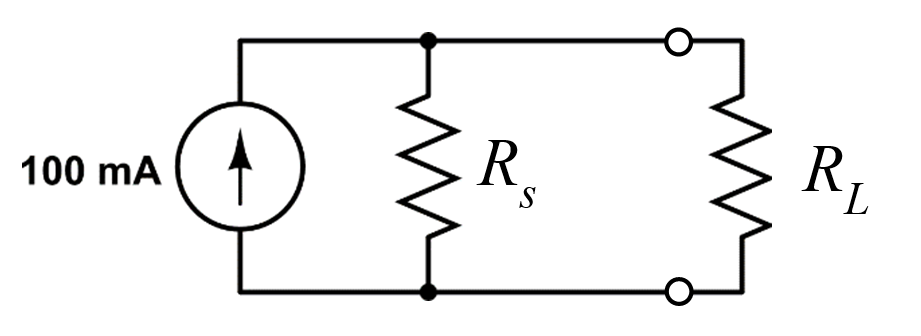
\includegraphics[width=0.5\textwidth]{figure.png}
\end{center}

% =========================================================
\begin{partquestion}{findvalue}
{Find the values for $R_S$ and $R_L$ that satisfy these constraints, assuming the resistors accurately match their marked values.}

\begin{answer}
There are 24 standard resistance values within a decade of values. We only need to consider one decade of values for the (smaller) $R_s$ since we will get identical results if we scale each resistor by a factor of ten:
\[
\frac{10R_s}{10R_s + 10R_L} = \frac{R_s}{R_s + R_L}.
\]

Since the dissipated current will be of the form $P = I^2 R$, we wish to make the resistances as small as possible to minimize this current dissipation, and we restrict our search to
\[
\qty{1}{\ohm} \le R_s \le \qty{91}{\ohm}.
\]

After choosing an $R_s$, we can find the optimal $R_L$ through the current divider relationship:
\[
I_L = \frac{R_s}{R_s + R_L}\left(\qty{100}{\milli\ampere}\right) = \qty{17}{\milli\ampere},
\]
so
\[
R_L = \frac{0.83}{0.17} R_s = 4.882\,R_s.
\]

Then we can select an actual resistance value that is closest to $4.882\,R_s$ and record the deviation. Note that as we get higher in the decade for $R_s$, the value for $R_L$ will extend into the next highest decade of resistor values, where everything is multiplied by a factor of 10.

We can manually step through 24 calculations, or we can write a small script to find the best pair. The MATLAB script below is not super-efficient because it looks at every pair of resistors to determine if it provides a better result than the best previously seen, but it is exceedingly simple to write and speed of execution is not critical since the search space is so small.

\clearpage
\begin{lstlisting}
R24=[10 11 12 13 15 16 18 20 22 24 27 30 33 36 39 43 47 51 56 62 68 75 82 91]/10;
pair=nchoosek([R24 R24*10],2);
dmin=1000;
for i=1:length(pair)
    d=abs(pair(i,1)/(pair(i,1)+pair(i,2))-.17);
    if d<dmin
        dmin=d;
        bestpair=pair(i,:);
    end
end
bestpair

\end{lstlisting}

Running this in MATLAB gives:

\begin{lstlisting}
bestpair =

    6.8000   33.0000
\end{lstlisting}
So we have $R_s=\qty{6.8}{\ohm}$ and $R_L=\qty{33}{\ohm}$.
\end{answer}
\end{partquestion}

% =========================================================
\begin{partquestion}{deviation}
{Calculate the \% deviation from the desired load current}

\begin{answer}
The two resistors above provide a load current of
\[I_L=\frac{\qty{6.8}{\ohm}}{\qty{6.8}{\ohm} + \qty{33}{\ohm}}(\qty{110}{\milli\ampere}) = \qty{17.085}{\milli\ampere}\]
which is a deviation of only
\[\frac{17.085-17}{17}\times100\% \approx0.5\%\]
\end{answer}
\end{partquestion}

% =========================================================
\begin{partquestion}{power}
{Calculate the total power dissipated in the circuit}

\begin{answer}
The total power dissipation is the sum of the power dissipated in each resistor. The current through the source resistor must be $100 - 17.085 = \qty{82.915}{\milli\ampere}$ and we can calculate
\[
P_{\text{total}} = P_{R_s} + P_{R_L} = {I_{R_S}}^2 R_S +{I_{R_L}}^2 R_L = (\qty{0.082915}{\ampere})^2(\qty{6.8}{\ohm})+\qty{0.017085}{\ampere}^2(\qty{33}{\ohm})
\]
which is only \qty{56.3}{\milli\watt}.
\end{answer}
\end{partquestion}

\end{mainquestion}